\documentclass[aspectratio=169]{beamer}
\usepackage[T1]{fontenc}
\usepackage[english]{babel}

\usetheme{Madrid}
\usecolortheme{default}

% \usepackage[utf8]{inputenc}
\usepackage[utf8]{vietnam}
\usepackage{amsmath, amssymb, amsfonts}
\usepackage{algorithm}
\usepackage[noend]{algpseudocode}
\usepackage{svg}
\usepackage{csquotes}
\usepackage{ragged2e}

\beamertemplatenavigationsymbolsempty

\usepackage[backend=biber, defernumbers=true,style=authortitle-ibid,citetracker=true,maxnames=1, minnames=1,sorting=none,doi=false,url=false]{biblatex}

\renewcommand*{\bibfont}{\normalfont\small}

\addbibresource{all-ref.bib}

% \title[SAAS]{Giải Thuật Đàn Kiến Tự Thích Ứng Cho Bài Toán Điều Hướng Thu Thập}
\title[SAAS]{Giải thuật đàn kiến tự thích ứng cho bài toán điều hướng thu thập}
\author[Việt, Vũ]{Lê Thế Việt - 20520093, Huỳnh Hoàng Vũ - 20520864}
\date[Tháng 1, 2024]{
    Giảng viên hướng dẫn: TS. Lương Ngọc Hoàng \\
    \vspace{0.3cm}
    Tháng 1, 2024}
\institute[UIT]
{
    Trường Đại học Công nghệ Thông tin, Đại học Quốc gia Thành phố Hồ Chí Minh \\
    \vspace{0.2cm}
    
\includegraphics[scale=0.135]{img/Logo_UIT_updated.jpg}
}

\AtBeginSection[]{
\begin{frame}
    % \frametitle{Table of Contents}
%     \tableofcontents[currentsection]
    \tableofcontents[sectionstyle=show/shaded, subsectionstyle=show/shaded/hide, subsubsectionstyle=show/shaded/hide]
\end{frame}
}
\AtBeginSubsection[]{
\begin{frame}
    % \frametitle{Table of Contents}
    \tableofcontents[sectionstyle=show/shaded, subsectionstyle=show/shaded/hide, subsubsectionstyle=show/shaded/hide]
\end{frame}
}
\begin{document}
\maketitle
\begin{frame}{Công bố khoa học}
    \justifying
    Vu Hoang Huynh, The Viet Le and Ngoc Hoang Luong. “Self-Adaptive Ant System with Hierarchical Clustering for the Thief Orienteering Problem”. In: Proceedings of the 12th International Symposium on Information and Communication Technology. SOICT 2023. ACM, Dec. 2023.
\end{frame}

\begin{frame}
    \frametitle{Mục lục}
    \tableofcontents[sectionstyle=show, subsectionstyle=hide, subsubsectionstyle=hide]
\end{frame}
\section{Bài toán Điều Hướng Thu Thập (ThOP)}
\subsection{Định nghĩa}
\begin{frame}{Bài toán Điều Hướng Thu Thập (ThOP)}
    \vspace*{-0.25cm}
    \begin{block}{Bài toán Điều Hướng Thu Thập (ThOP)}
        \footnotesize Bài toán Điều Hướng Thu Thập (\textbf{Th}ief \textbf{O}rienteering \textbf{P}roblem, ThOP) \footnotemark là bài toán tối ưu hóa \textbf{đa thành phần} bao gồm 2 thành phần, \textbf{bài toán Điều Hướng} (\textbf{O}rienteering \textbf{P}roblem, OP) và \textbf{bài toán Ba Lô} (\textbf{K}napsack \textbf{P}roblem, KP).
    \end{block}
    \footnotetext{\fullcite{8477853}}
\end{frame}

\begin{frame}{Bài toán Điều Hướng Thu Thập (ThOP)}
    \onslide<1->{
        \vspace{-0.2cm}
        \begin{columns}
            \hspace{0.17cm}
            \begin{column}{0.55\textwidth}
                \begin{block}{\small Bài toán Điều Hướng (OP)}
                    \justifying
                    \small OP là một bài toán định tuyến với mục tiêu \textbf{xác định một con đường} trong tập thành phố cho trước, nhằm \textbf{tối đa hóa tổng điểm đạt được} từ các thành phố đi qua, trong khi vẫn \textbf{đảm bảo giới hạn thời gian}.
                \end{block}
            \end{column}

            \begin{column}{0.45\textwidth}
                \begin{center}
                    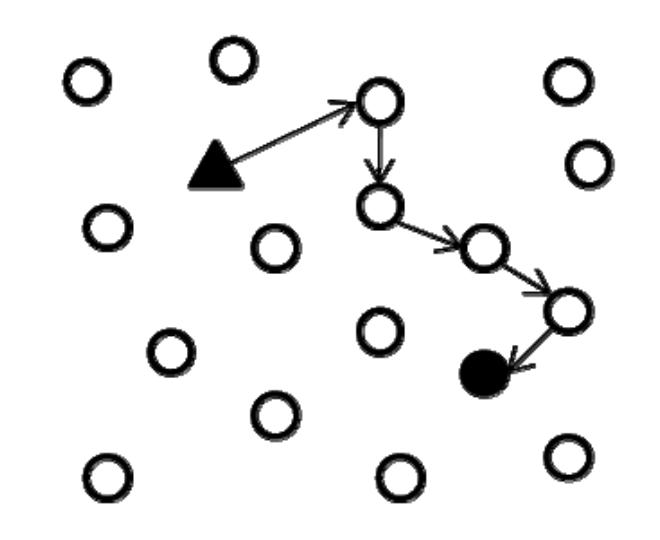
\includegraphics[scale=0.25]{img/orienteering.jpg}
                \end{center}
            \end{column}
        \end{columns}
        \vspace{0.4cm}
    }
    \onslide<2->{
        \begin{columns}
            \hspace{0.17cm}
            \begin{column}{0.55\textwidth}
                \begin{block}{\small Bài toán Ba Lô (KP)}
                    \justifying
                    \small KP là một bài toán tối ưu hóa tổ hợp với mục tiêu \textbf{lựa chọn nhặt các vật phẩm} trong tập vật phẩm cho trước, nhằm \textbf{tối đa hóa lợi nhuận thu thập được} từ các vật phẩm, trong khi vẫn \textbf{đảm bảo giới hạn sức chứa}.
                \end{block}
            \end{column}

            \begin{column}{0.45\textwidth}
                \begin{center}
                    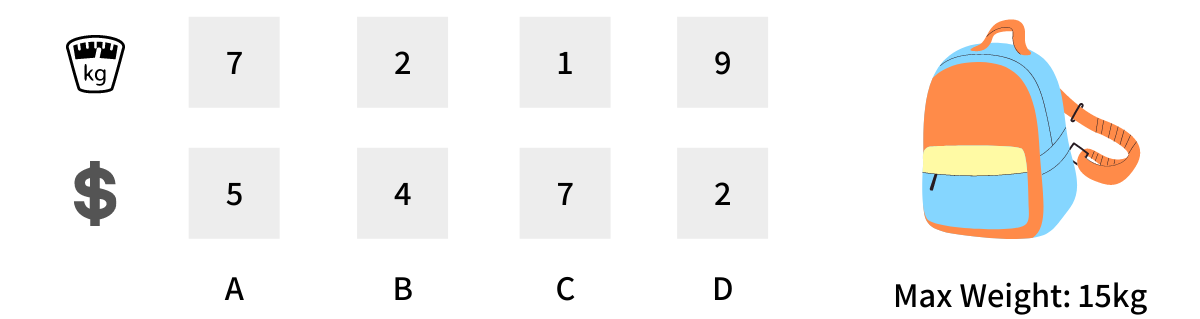
\includegraphics[scale=0.15]{img/knapsack.png}
                \end{center}
            \end{column}
        \end{columns}
    }

\end{frame}

\subsection{Ví dụ}
\begin{frame}{ThOP - Ví dụ}
    \begin{columns}
        \begin{column}{0.5\textwidth}
            \begin{center}
                \only<1>{
                    \includesvg[inkscapelatex=false, width=\columnwidth]{img/Example1-v2.svg}
                }
                \only<2>{
                    \includesvg[inkscapelatex=false, width=\columnwidth]{img/Example2-v2.svg}
                }
                \only<3>{
                    \includesvg[inkscapelatex=false, width=\columnwidth]{img/Example3-v2.svg}
                }
                \only<4>{
                    \includesvg[inkscapelatex=false, width=\columnwidth]{img/Example4-v2.svg}
                }
            \end{center}

        \end{column}

        \begin{column}{0.45\textwidth}
            \only<1>{
                \vspace{-5cm}
                \begin{block}{\small Ràng buộc}
                    \footnotesize
                    \begin{itemize}
                        \item $n = 4, m = 5$
                        \item $v_{min} = 0.1, v_{max}  = 1.0, W = 3, T = 75$
                    \end{itemize}

                \end{block}
            }
            \only<2>{

                \begin{block}{\small Ràng buộc}
                    \footnotesize
                    \begin{itemize}
                        \item $n = 4, m = 5$
                        \item $v_{min} = 0.1, v_{max}  = 1.0, W = 3, T = 75$
                    \end{itemize}

                \end{block}
                \begin{block}{\small Lời giải}
                    \footnotesize
                    \begin{itemize}
                        \item $\pi = \langle 1 \rangle$
                        \item $p = \langle 0, 0, 0, 0 ,0 \rangle$
                    \end{itemize}
                \end{block}

                \begin{block}{\small Thuộc tính}
                    \footnotesize
                    \begin{itemize}
                        \item $p = 0$
                        \item $w = 0$
                        \item $v = v_{max} = 1.0$
                        \item $t = 0$
                    \end{itemize}

                \end{block}
            }

            \only<3>{

                \begin{block}{\small Ràng buộc}
                    \footnotesize
                    \begin{itemize}
                        \item $n = 4, m = 5$
                        \item $v_{min} = 0.1, v_{max}  = 1.0, W = 3, T = 75$
                    \end{itemize}

                \end{block}
                \begin{block}{\small Lời giải}
                    \footnotesize
                    \begin{itemize}
                        \item $\pi = \langle 1, 3 \rangle$
                        \item $p = \langle 0, 0, 0 ,0 ,0 \rangle$
                    \end{itemize}
                \end{block}

                \begin{block}{\small Thuộc tính}
                    \footnotesize
                    \begin{itemize}
                        \item $p = 0$
                        \item $w = 0$
                        \item $v = v_{max} = 1.0$
                              \pause
                        \item $t = d_{1,3} / v = 6 / 1.0 = 6$
                    \end{itemize}

                \end{block}
            }

            \only<4>{

                \begin{block}{\small Ràng buộc}
                    \footnotesize
                    \begin{itemize}
                        \item $n = 4, m = 5$
                        \item $v_{min} = 0.1, v_{max}  = 1.0, W = 3, T = 75$
                    \end{itemize}

                \end{block}
                \begin{block}{\small Lời giải}
                    \footnotesize
                    \begin{itemize}
                        \item $\pi = \langle 1, 3, 4 \rangle$
                        \item $p = \langle 0, 0, 1 ,0 ,0 \rangle$
                    \end{itemize}
                \end{block}

                \begin{block}{\small Thuộc tính}
                    \footnotesize
                    \begin{itemize}
                        \item $p = 100$
                        \item $w = 0 + w_{3} = 3$
                              \pause
                        \item $v = v_{max} - w (v_{max} - v_{min}) / W = 0.1$
                              \pause
                        \item $t = t + d_{3,4} / v = 6 + 5 / 0.1 = 56$
                    \end{itemize}

                \end{block}
            }
        \end{column}
    \end{columns}
\end{frame}

% \subsection{Motivation}
% \begin{frame}{Motivation}
%     \begin{block}{Theoretical Motivation}
%         \vspace{0.2cm}
%         \begin{itemize}
%             \item ThOP can be a benchmark for evaluating and comparing optimization methods.
%             \item ThOP can contribute to solving its component problems OP and KP, even TTP and TSP.
%         \end{itemize}
%         \vspace{0.2cm}
%     \end{block}
%     \pause
%     \begin{block}{Practical Motivation}
%         \vspace{0.2cm}
%         ThOP can be generalized to solve real-world problems:
%         \begin{itemize}
%             \item Planing a route for a vehicle to collect packages in multiple warehouses with time constraints and capacity limits.
%             \item Planing a route for a rescue team to visit a set of locations to collect supplies and rescue victims.
%         \end{itemize}
%         \vspace{0.2cm}
%     \end{block}
% \end{frame}


\subsection{ThOP benchmark}
\begin{frame}{ThOP benchmark}
    \begin{block}{ThOP Benchmark}
        \justifying
        ThOP benchmark là tập hợp gồm 432 trường hợp của bài toán. Các trường hợp mang tính chất khác nhau về:
        \begin{itemize}
            \item Số lượng thành phố: 51, 107, 280, hoặc 1000.
            \item Số lượng vật phẩm tại mỗi thành phố: 01, 03, 05, hoặc 10.
            \item Mối quan hệ giữa cân nặng và lợi nhuận: uncorrelated (unc), uncorrelated with similar weights (usw), hoặc bounded and strongly correlated (bsc).
            \item Kích thước balo: 01, 05, hoặc 10 lần kích thước nhỏ nhất.
            \item Thời gian di chuyển tối đa: 50\%, 75\%, hoặc 100\%.
        \end{itemize}
    \end{block}
\end{frame}

\section{Các công trình liên quan}
\begin{frame}{Các công trình liên quan}
    \begin{block}{Các thuật toán trước đây cho ThOP}
        \small
        \begin{itemize}
            % \item Mixed Integer Non-Linear Programming (MINLP) \footnotemark[1]
            % \item Iterated local search algorithm (ILS) \footnotemark[1]
            % \item Biased random-key genetic algorithm (BRKGA) \footnotemark[1]
            % \item Genetic Algorithm (GA) \footnotemark
            % \item Ant Colony Optimization algorithm (ACO) \footnotemark
            % \item Max-Min Ant System algorithm (ACO++) \footnotemark
            \item Tìm Kiếm Cục Bộ Tuần Tự (\textbf{I}terated \textbf{L}ocal \textbf{S}earch, ILS) \footnotemark[1].
            \item Thuật Giải Di Truyền Điểm Thiên Lệch Ngẫu Nhiên (\textbf{B}iased \textbf{R}andom-\textbf{K}ey \textbf{G}enetic \textbf{A}lgorithm, BRKGA) \footnotemark[1].
            \item Thuật Giải Di Truyền (\textbf{G}enetic \textbf{A}lgorithm, GA) \footnotemark.
            \item Giải Thuật Tối Ưu Hóa Đàn Kiến (\textbf{A}nt \textbf{C}olony \textbf{O}ptimization, ACO) \footnotemark.
            \item ACO++ \footnotemark.
        \end{itemize}
    \end{block}
    \footnotetext[2]{\fullcite{9185848}}
    \footnotetext[3]{\fullcite{CHAGAS2020708}}
    \footnotetext[4]{\fullcite{Chagas2021}}
\end{frame}


\section{Thuật toán tân tiến trước đây (ACO++)}
\subsection{Tổng quan}
\begin{frame}{Ý tưởng của ACO}
    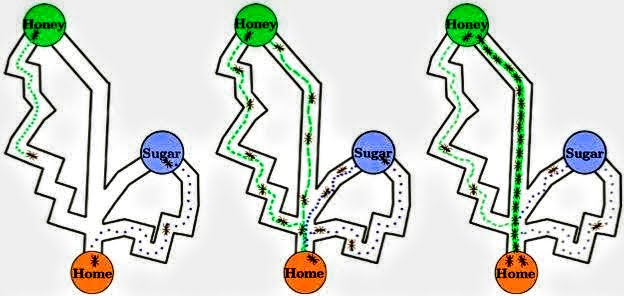
\includegraphics[width=\columnwidth]{img/ACO concept.jpg}
\end{frame}
\begin{frame}{Tổng quan ACO++}
    \begin{columns}
        \begin{column}{0.35\textwidth}
            \vspace{-0.2cm}
            \begin{center}
                \begin{figure}[htbp]
                    \centering
                    \includesvg[inkscapelatex=false, width=0.9\columnwidth]{img/ACO++.svg}  \\
                    % \vspace{0.4cm}
                    % \tiny \textbf{Tổng quan ACO++}
                    % \label{fig:aco++fc}
                \end{figure}
            \end{center}
        \end{column}
        \begin{column}{0.5\textwidth}
            \begin{block}{ACO++}
                \footnotesize
                \begin{itemize}
                    \justifying
                    \vspace{0.1cm}
                    \item ACO++ được Chagas và Wagner đề xuất và trở thành thuật toán tân tiến cho ThOP.
                    \vspace{0.1cm}
                    \item ACO++ là sự kết hợp của Hệ thống Kiến Max-Min Heuristic nhặt ngẫu nhiên và Tìm kiếm cục bộ.
                    \vspace{0.1cm}
                    \item ACO++ vượt trội hơn các thuật toán trước đây trên 95\% benchmark.
                    \vspace{0.1cm}
                \end{itemize}
            \end{block}
        \end{column}
    \end{columns}
\end{frame}

% \subsection{Heuristic nhặt ngẫu nhiên}
\begin{frame}{Heuristic nhặt ngẫu nhiên của ACO++}
    \onslide<1-> {
    \begin{block}{Điểm vật phẩm $s_i$}
        $$s_i = \frac{p_i^\theta}{w_i^\delta * d_i^\gamma}$$
    \end{block}
    }
    \only<1> {
    \begin{block}{Heuristic nhặt ngẫu nhiên (Randomized Packing Heuristic)}
        \begin{enumerate}
            \justifying
            \vspace{0.1cm}
            \item Tính điểm cho các vật phẩm.
            \vspace{0.1cm}
            \item Xem xét vật phẩm có điểm cao nhất tiếp theo.
            \vspace{0.1cm}
            \item Nếu nhặt thêm vật phẩm không làm vi phạm ràng buộc, thêm nó vào balo.
            \vspace{0.1cm}
            \item Nếu chưa xem xét qua tất cả vật phẩm, quay lại Bước 2.
            \vspace{0.1cm}
        \end{enumerate}
    \end{block}
    }
    % \only<2> {
    % \begin{block}{Trong đó}
    %     \begin{itemize}
    %         % \justifying
    %         \vspace{0.1cm}
    %         \item $p_i$: Lợi nhuận của vật phẩm $i$.
    %         \vspace{0.1cm}
    %         \item $w_i$: Trọng lượng của vật phẩm $i$.
    %         \vspace{0.1cm}
    %         \item $d_i$: Độ dài đường đi từ thành phố chứa vật phẩm $i$ đến thành phố cuối cùng theo thứ tự đường đi đang xét.
    %         \vspace{0.1cm}
    %         \item $\theta$, $\delta$, $\gamma$: Giá trị được tạo ngẫu nhiên trong khoảng [0,1].
    %         \vspace{0.1cm}
    %     \end{itemize}
    % \end{block}
    % }
\end{frame}


\subsection{Nhược điểm}

\begin{frame}{Nhược điểm của ACO++}
    \begin{block}{Nhược điểm của ACO++}
        \begin{enumerate}
            \vspace{0.1cm}
            \item Heuristic nhặt vật phẩm lệ thuộc nhiều vào yếu tố ngẫu nhiên.
            \vspace{0.1cm}
            \item 
            \vspace{0.1cm}
        \end{enumerate}
    \end{block}
\end{frame}

\begin{frame}{Heuristic nhặt vật phẩm lệ thuộc nhiều vào ngẫu nhiên}
    \begin{block}{Điểm vật phẩm $s_i$}
        $$s_i = \frac{p_i^\theta}{w_i^\delta * d_i^\gamma}$$
    \end{block}
    
    \begin{block}{Trong đó}
        \begin{itemize}
            \justifying
            \vspace{0.1cm}
            \item $p_i$: Lợi nhuận của vật phẩm $i$.
            \vspace{0.1cm}
            \item $w_i$: Trọng lượng của vật phẩm $i$.
            \vspace{0.1cm}
            \item $d_i$: Độ dài đường đi từ thành phố chứa vật phẩm $i$ đến thành phố cuối cùng theo thứ tự đường đi đang xét.
            \vspace{0.1cm}
            \item \textbf{$\theta$, $\delta$, $\gamma$: Giá trị được tạo \textcolor{red}{ngẫu nhiên} trong khoảng [0,1].}
            \vspace{0.1cm}
        \end{itemize}
    \end{block}
\end{frame}

\begin{frame}{Nhược điểm của ACO++}
    \begin{block}{Nhược điểm của ACO++}
        \begin{enumerate}
            \vspace{0.1cm}
            \item Heuristic nhặt vật phẩm lệ thuộc nhiều vào yếu tố ngẫu nhiên.
            \vspace{0.1cm}
            \item Hiệu suất nhạy với giá trị siêu tham số. Các siêu tham số cần được điều chỉnh riêng cho mỗi 9 trường hợp.
            \vspace{0.1cm}
        \end{enumerate}
    \end{block}
\end{frame}

\begin{frame}{Hiệu suất phụ thuộc nhiều vào siêu tham số}
    \begin{block}{Quá trình điều chỉnh siêu tham số tốn kém}
        \begin{itemize}
            % \justifying
            \vspace{0.1cm}
            \item ACO++ đòi hỏi một quá trình điều chỉnh tốn kém để đạt được kết quả vượt trội.
            \vspace{0.1cm}
            \item 240.000 thí nghiệm đã được tiến hành để điều chỉnh 48 bộ siêu tham số cho 48 nhóm trường hợp.
            \vspace{0.1cm}
            \item Mỗi nhóm bao gồm 9 trường hợp.
            \vspace{0.1cm}
        \end{itemize}
    \end{block}

    % \begin{block}{Thí nghiệm về độ nhạy tham số của ACO++}
    %     \justifying
    %     Các thí nghiệm của chúng tôi được thực hiện trên hai nhóm trường hợp từ ThOP benchmark:
    %     \begin{itemize}
    %         \item \texttt{a280\_01\_unc}: 280 thành phố, 1 vật phẩm mỗi thành phố, lợi nhuận không tương quan với trọng lượng.
    %         \item \texttt{dsj1000\_01\_unc}: 1000 thành phố, 1 vật phẩm mỗi thành phố, lợi nhuận không tương quan với trọng lượng.
    %     \end{itemize}
    %     \vspace{0.1cm}
    % \end{block}

\end{frame}
\begin{frame}{Hiệu suất phụ thuộc nhiều vào siêu tham số}
    \begin{columns}
        \begin{column}{0.45\textwidth}
            \vspace{-0.3cm}
            \footnotesize
            \begin{block}{\footnotesize Thí nghiệm 1}
                Sử dụng bộ siêu tham số được điều chỉnh riêng cho nhóm trường hợp.
            \end{block}
            \begin{block}{\footnotesize Thí nghiệm 2}
                Hoán đổi bộ siêu tham số của hai nhóm trường hợp.
            \end{block}
            \begin{block}{\footnotesize Thí nghiệm 3}
                Tăng 3\% cho $\alpha$, $\beta$, $\rho$ và tăng 1 cho số lần thử nhặt vật phẩm.
            \end{block}
            \begin{block}{\footnotesize Thí nghiệm 4}
                Lấy trung bình của 48 bộ siêu tham số.
            \end{block}
        \end{column}
        \begin{column}{0.45\textwidth}
            % 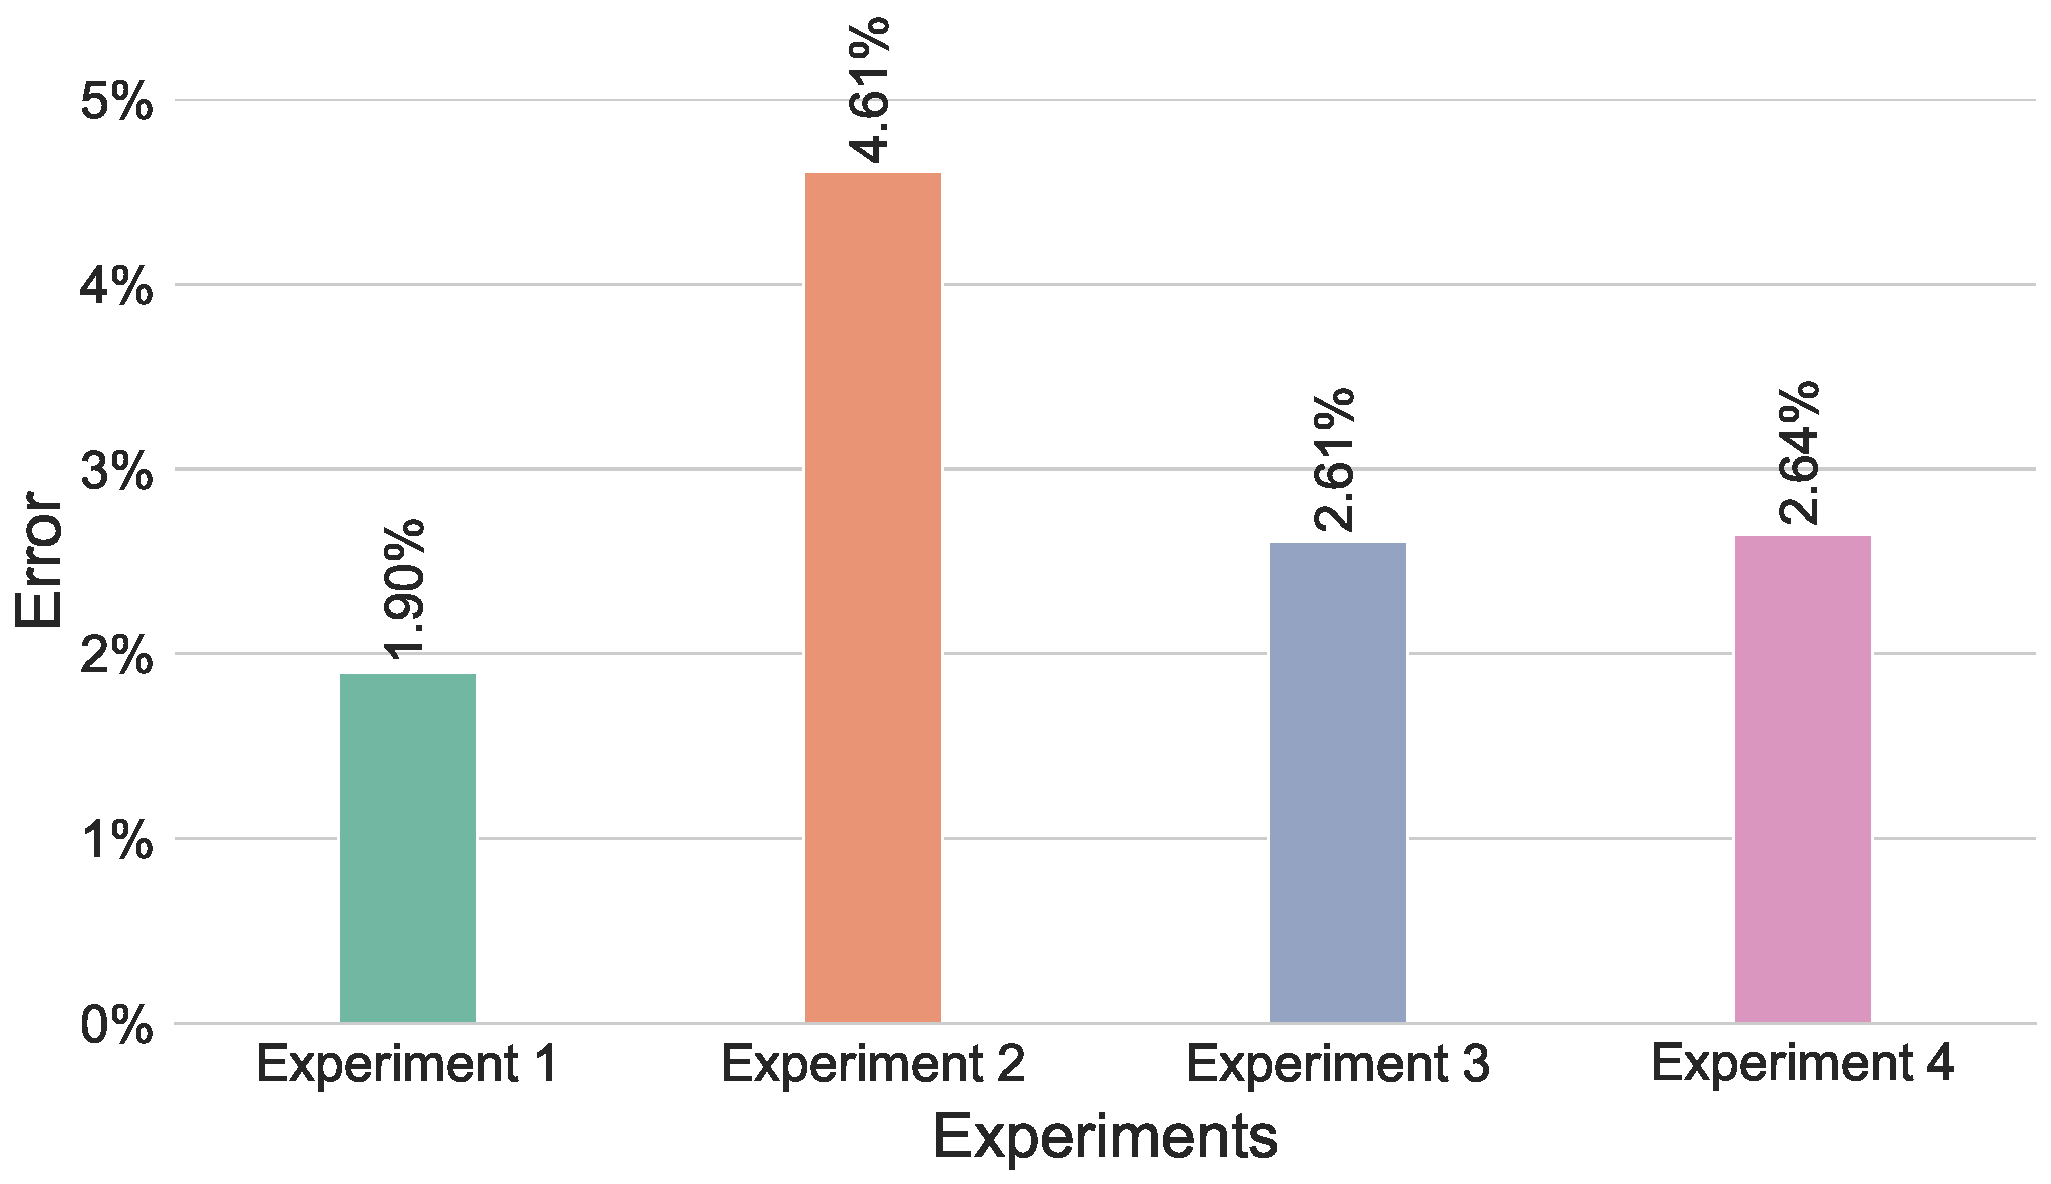
\includegraphics[width=\linewidth]{img/sensitive_error_rate.pdf}
            \begin{figure}[h]
                \centering
                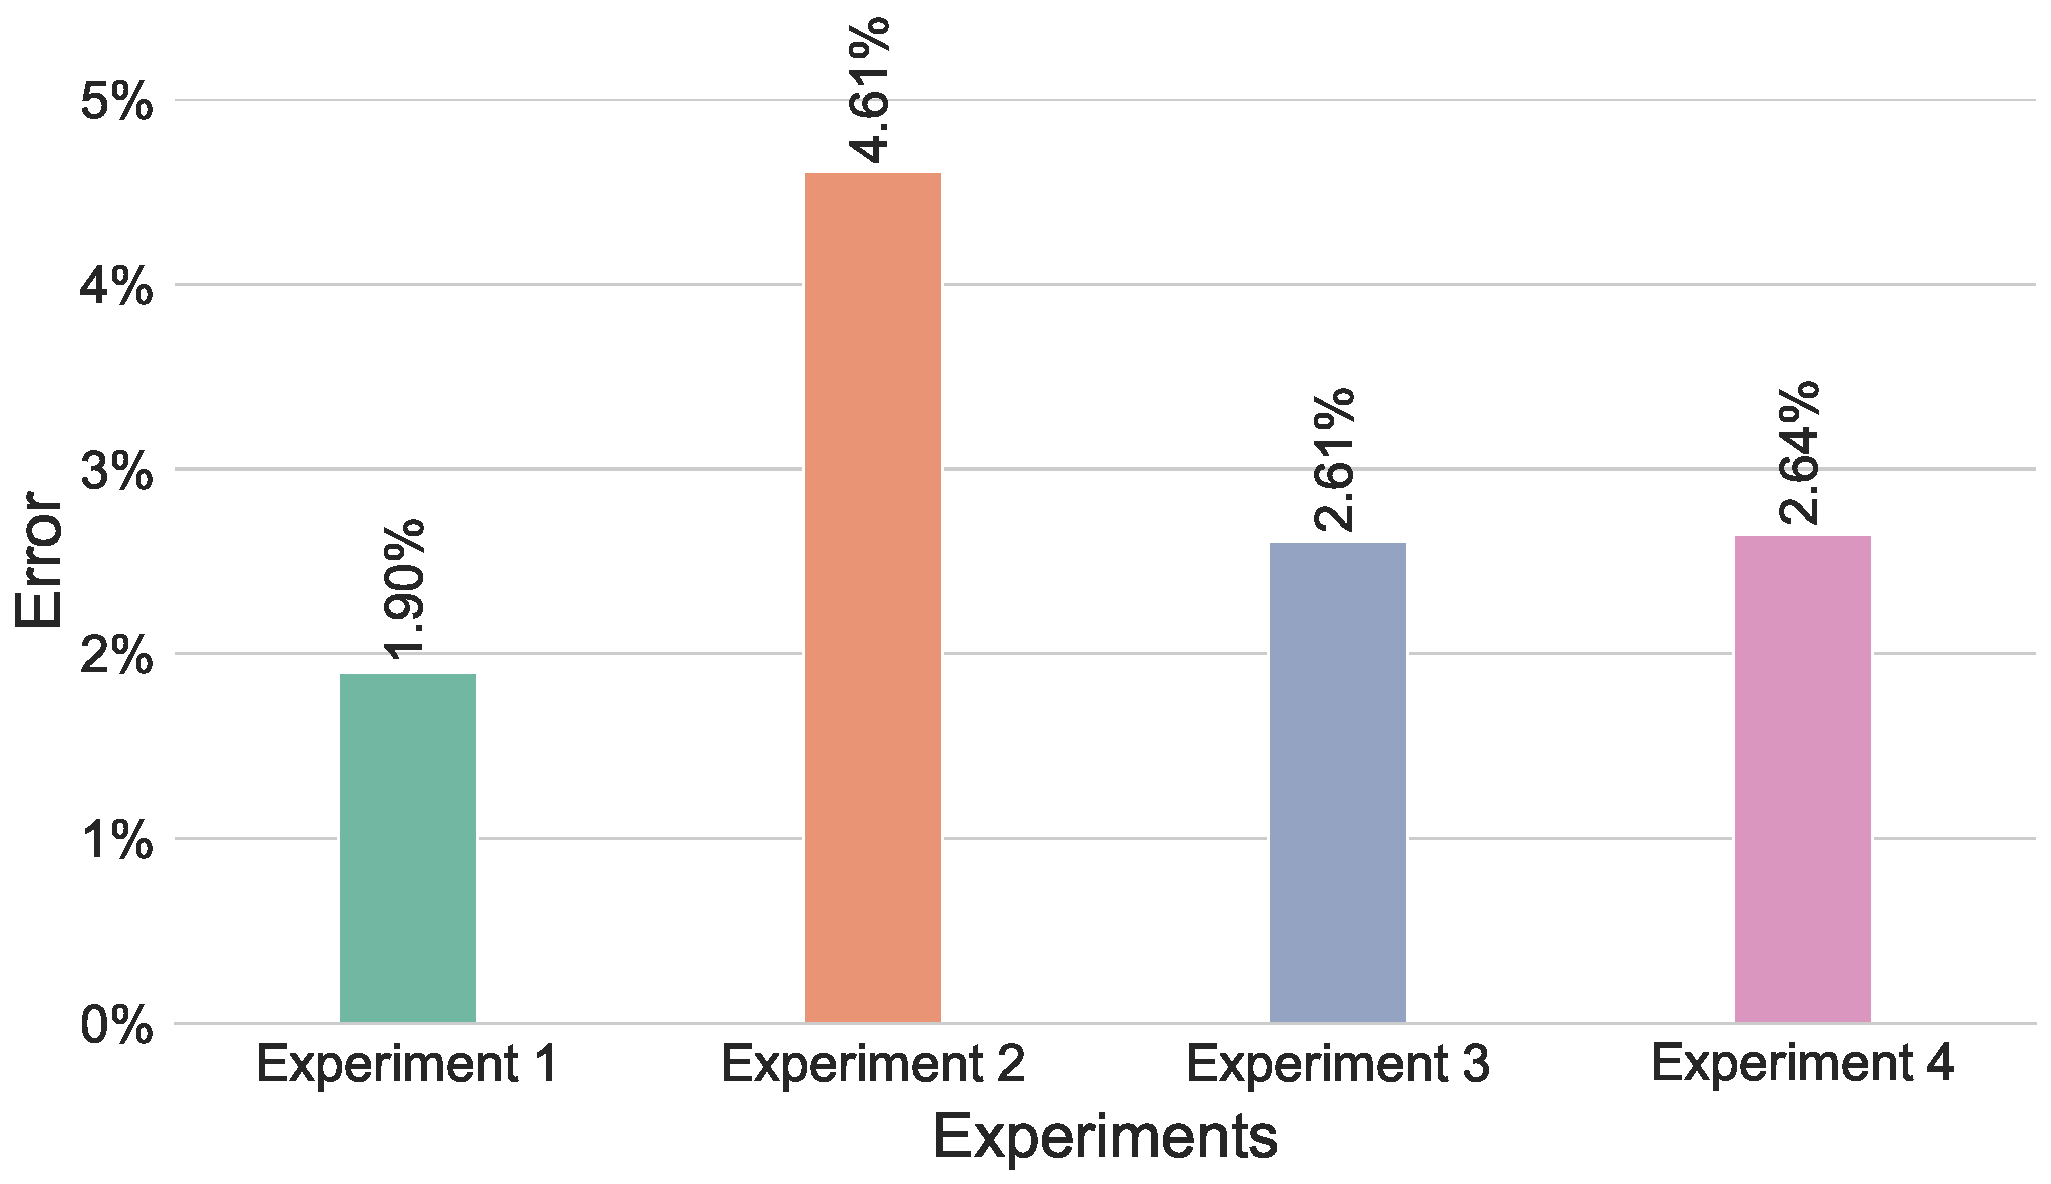
\includegraphics[width=\linewidth]{img/sensitive_error_rate.pdf}
                % \caption{\footnotesize Mean errors of results of 4 ACO++ experiments with different parameter sets on 18 instances belonging to 2 ThOP instance groups.}
                \caption{\footnotesize\justifying Sai số trung bình của kết quả từ 4 thí nghiệm ACO++ với các bộ tham số khác nhau trên 18 trường hợp thuộc 2 nhóm trường hợp ThOP. Nhỏ hơn là tốt hơn.}
                \label{fig:sensitive}
            \end{figure}
        \end{column}
    \end{columns}
\end{frame}

% \begin{frame}{Nhược điểm của ACO++}
%     \begin{block}{Nhược điểm của ACO++}
%         \begin{enumerate}
%             \vspace{0.1cm}
%             \item Heuristic nhặt vật phẩm lệ thuộc nhiều vào yếu tố ngẫu nhiên.
%             \vspace{0.1cm}
%             \item Hiệu suất nhạy với giá trị siêu tham số. Các siêu tham số cần được điều chỉnh riêng cho mỗi 9 trường hợp.
%             \vspace{0.1cm}
%         \end{enumerate}
%     \end{block}
% \end{frame}


\section{Giải thuật đàn kiến tự thích ứng (SAAS)}
\begin{frame}{Tổng quan thuật toán SAAS}
    \begin{block}{Đóng góp của đề tài}
        \begin{itemize}
            \justifying
            \vspace{0.1cm}
            \item Chúng tôi đề xuất Giải Thuật Đàn Kiến Tự Thích Ứng (\textbf{S}elf-\textbf{A}daptive \textbf{A}nt \textbf{S}ystem, SAAS), là phiên bản mở rộng của ACO++.
            \vspace{0.1cm}
            \item SAAS có thể điều chỉnh các tham số của mình dựa trên đặc điểm riêng biệt của trường hợp bài toán và quá trình tìm kiếm.
            \vspace{0.1cm}
            \item Đồng thời, nó có độ phức tạp thời gian thấp hơn ACO++ ở giai đoạn kiến chọn thành phố và giai đoạn bay hơi pheromone.
            \vspace{0.1cm}
        \end{itemize}
    \end{block}
\end{frame}

\begin{frame}{Tổng quan thuật toán SAAS}
    \vspace{0.1cm}
    \centering
    \includesvg[inkscapelatex=false, width=0.85\columnwidth]{img/SAAS-HC_chú thích.svg}
\end{frame}


\subsection{Cơ chế tự thích ứng với CMA-ES}
\begin{frame}{CMA-ES}
    \begin{columns}
        \begin{column}{0.6\textwidth}
            \hspace{0.2cm}
            \begin{block}{Giới thiệu}
                \justifying
                \vspace{0.1cm}
                CMA-ES\footnotemark (\textbf{C}ovariance \textbf{M}atrix \textbf{A}daptation \textbf{E}volution \textbf{S}rategy, Chiến lược Tiến hóa Thích ứng Ma trận Hiệp Phương Sai) là một phương pháp tối ưu hóa số, ngẫu nhiên, \textbf{không sử dụng đạo hàm} cho các bài toán tối ưu hóa \textbf{phi tuyến tính} hoặc \textbf{không lồi} trên không gian \textbf{liên tục}.
                \vspace{0.1cm}
            \end{block}
        \end{column}

        \begin{column}{0.4\textwidth}
            \vspace{-0.3cm}
            \begin{figure}
                \centering
                \includegraphics[width=0.7\columnwidth]{img/simplified_CMA-ES.pdf}
                \footnotesize
                \caption{Sơ đồ đơn giản hóa CMA-ES.}
            \end{figure}
        \end{column}
    \end{columns}
    \footnotesize \footnotemark[5]{\fullcite{Hansen2006}}
\end{frame}

\begin{frame}{Cơ chế tự thích ứng với CMA-ES}
    \vspace{0.1cm}
    \centering
    \includesvg[inkscapelatex=false, width=0.85\columnwidth]{img/CMA-ES Flowchart-v3.svg}
\end{frame}


\subsection{Sử dụng thông tin sự đa dạng về lợi nhuận để thích ứng}
\begin{frame}{Sử dụng thông tin sự đa dạng về lợi nhuận để thích ứng}
    \vspace{0.1cm}
    \centering
    \includesvg[inkscapelatex=false, width=0.85\columnwidth]{img/Adaptive Flowchart-v3.svg}
\end{frame}

\begin{frame}{Sử dụng thông tin sự đa dạng về lợi nhuận để thích ứng}
    \begin{block}{\small Ý tưởng chính}
        \small 
        Lấy cảm hứng từ thuật toán AACO-NC\footnotemark, chúng tôi sử dụng thông tin sự đa dạng về lợi nhuận để thay đổi linh hoạt cả tỷ lệ bay hơi pheromone và số lượng kiến cho mỗi cá thể của CMA-ES.
        \vspace{0.1cm}
    \end{block}
    \begin{block}{\small Thông tin sự đa dạng về lợi nhuận}
        \small 
        \begin{equation}\label{eq:entropy_prob}
            p_{i} = \frac{\text{\#số lần xuất hiện}(P_{i})}{n_{\text{ants}}}
        \end{equation}
        \begin{equation}\label{eq:entropy}
            \begin{split}
                S = \{P\  |\ \text{$P$ là giá trị}&\text{ độc nhất được tìm bởi đàn kiến hiện tại}\} ,\\
                H &= -\sum_{i=1}^{|S|} p_{i} \cdot \log_2 p_{i}
            \end{split}
        \end{equation}
    \end{block}
    \footnotetext[6]{\fullcite{STODOLA2022101056}}
\end{frame}

\begin{frame}{Sử dụng thông tin sự đa dạng về lợi nhuận để thích ứng}
    \begin{block}{Thích ứng tỷ lệ bay hơi pheromone}
        \vspace{0.1cm}
        \begin{itemize}
            \item Tỷ lệ bay hơi \textbf{tăng khi} lợi nhuận \textbf{đa dạng cao} và \textbf{giảm khi} lợi nhuận \textbf{đa dạng thấp}.
        \end{itemize}
        \begin{equation}\label{eq:adaptrho}
            \rho = \rho_{\textbf{min}} \textbf{ + } (\rho_{\text{max}} - \rho_{\text{min}}) \cdot \frac{H - H_{\text{min}}}{H_{\text{max}} - H_{\text{min}}}.
        \end{equation}
        \vspace{0.1cm}
    \end{block}
    \begin{block}{Thích ứng số lượng kiến cho mỗi cá thể CMA-ES}
        \vspace{0.1cm}
        \begin{itemize}
            \item Trái ngược với tỷ lệ bay hơi, giá trị của $n_{indv}$ \textbf{tăng khi} lợi nhuận \textbf{đa dạng thấp} để khuyến khích khám phá và \textbf{giảm khi} lợi nhuận \textbf{đa dạng cao} để tập trung khai thác.
        \end{itemize}
        \begin{equation} \label{eq:adaptants}
            n_{\text{indv}} = n_{\text{indv\_}\textbf{max}} \textbf{ - } (n_{\text{indv\_max}} - n_{\text{indv\_min}}) \cdot \frac{H - H_{\text{min}}}{H_{\text{max}} - H_{\text{min}}}.
        \end{equation}
        \vspace{0.1cm}
    \end{block}
\end{frame}


\begin{frame}{Các tham số được điều khiển}
    \vspace{-0.5cm}
    \begin{table}
        \small
        \caption{Danh sách các tham số được điều khiển bởi cơ chế điều khiển tham số.}
        \label{tab:control_param}
        \begin{tabular}{l|l|l}
            \hline
            Tham số                                & Cơ chế điều khiển tham số & Khoảng giá trị                                            \\
            \hline
            % $n\_ants$                   &   adaptive                    \\
            $\alpha$                                 & Tự thích ứng               & [0, 1]                                           \\
            $\beta$                                  & Tự thích ứng               & [0, 1]                                           \\
            $\rho_{\text{min}}$, $\rho_{\text{max}}$ & Tự thích ứng               & [0, 1]                                           \\
            $\theta$                                 & Tự thích ứng               & [0, 1]                                           \\
            $\delta$                                 & Tự thích ứng               & [0, 1]                                           \\
            $\gamma$                                 & Tự thích ứng               & [0, 1]                                           \\
            $n_{\text{indv}}$                        & Thích ứng                    & [$n_{\text{indv\_max}}$, $n_{\text{indv\_min}}$] \\
            $\rho$                                   & Thích ứng                    & [$\rho_{\text{min}}, \rho_\text{{max}}$]         \\
            \hline
        \end{tabular}
    \end{table}

    \vspace{0.2cm}
    \begin{itemize}
        \item Ba số mũ ngẫu nhiên $\theta, \delta, \gamma$ trong Heuristic nhặt vật phẩm đã được điều chỉnh bởi CMA-ES.
    \end{itemize}
\end{frame}


\subsection{Kiến di chuyển trên cây cụm thứ bậc}
\begin{frame}{Kiến di chuyển trên cây cụm thứ bậc}
    \vspace{0.1cm}
    \centering
    \includesvg[inkscapelatex=false, width=0.85\columnwidth]{img/Tree Flowchart-v3.svg}
\end{frame}

\begin{frame}{Kiến di chuyển trên cây cụm thứ bậc}
    \begin{columns}
        \begin{column}{0.55\textwidth}
            \begin{block}{Ý tưởng chính}
                \vspace{0.1cm}
                \begin{itemize}
                    \justifying
                    % \item We use hierarchical clustering to build the tree architecture.
                    % \item Each city has its own cluster tree that represents the edges going to $n$ cities.
                    % \item Ants will traverse cluster trees instead of moving directly from one city to another.
                    % \item This way, we can reduce the time complexity of choosing the next city to $\Theta(\log n)$.
                    \item Chúng tôi sử dụng phân cụm thứ bậc (hierarchical clustering) để xây dựng kiến trúc cây.
                    \item Mỗi thành phố có một cây cụm thứ bậc đại diện cho các cạnh đi đến $n$ thành phố.
                    \item Kiến sẽ duyệt cây từ gốc đến lá thay vì di chuyển trực tiếp từ thành phố đến thành phố.
                    \item Bằng cách này, giai đoạn kiến chọn thành phố tiếp theo sẽ có độ phức tạp $\Theta(\log n)$.
                \end{itemize}
                \vspace{0.1cm}
            \end{block}
        \end{column}
        \begin{column}{0.45\textwidth}
            \begin{figure}
                \vspace{0.1cm}
                \centering
                \includesvg[inkscapelatex=false, width=0.85\columnwidth]{img/Cluster tree-v2.svg}
                \caption{Ví dụ cây cụm thứ bậc.}
            \end{figure}
        \end{column}
    \end{columns}
\end{frame}


\subsection{Bay hơi lười biếng}
\begin{frame}{Bay hơi lười biếng}
    \vspace{0.1cm}
    \centering
    \includesvg[inkscapelatex=false, width=0.85\columnwidth]{img/Lazy-v3.svg}
\end{frame}

\begin{frame}{Bay hơi lười biếng}
    \begin{block}{Ý tưởng chính}
        \begin{itemize}
            \justifying
            \vspace{0.1cm}
            \item Nguyên tắc cốt lõi của bay hơi lười biếng là ghi nhận trạng thái mong muốn và trạng thái lịch sử.
            \vspace{0.1cm}
            \item Trạng thái mong muốn bao gồm số lần bay hơi pheromone mong muốn.
            \vspace{0.1cm}
            \item Mỗi cạnh sẽ có trạng thái lịch sử riêng, bao gồm số lần nồng độ pheromone của cạnh thực sự được bay hơi.
            \vspace{0.1cm}
            \item Bằng cách so sánh trạng thái mong muốn và trạng thái lịch sử, ta có thể xác định nồng độ pheromone với số lần bay hơi mong muốn khi cần thiết.
            \vspace{0.1cm}
        \end{itemize}
    \end{block}
\end{frame}

\begin{frame}{Tổng quan thuật toán SAAS}
    \vspace{0.1cm}
    \centering
    \includesvg[inkscapelatex=false, width=0.85\columnwidth]{img/SAAS-HC_chú thích.svg}
\end{frame}

\section{Thực nghiệm}
\begin{frame}{Thực nghiệm}
    \vspace{-0.3cm}
    \begin{block}{Để có sự so sánh công bằng}
    \begin{itemize}
        \item Thực nghiệm được tiến hành trên \textbf{cùng phần cứng}.
        \item Các thuật toán có \textbf{cùng giới hạn thời gian chạy}.
    \end{itemize}
    \end{block}
    \begin{block}{Điều chỉnh siêu tham số}
        \begin{itemize}
        \justifying
            % \item BRKGA, ACO, and ACO++ used the same parameters fine-tuned in the ACO++ paper.
            % \item 240,000 experiments were performed for tuning each algorithm. ILS had no parameters to fine-tune.
            % \item evosax\footnotemark framework was used to tune SAAS hyperparameters.
            % \item 45,000 experiments were performed to tune SAAS for all benchmark instances.
            \vspace{0.1cm}
            \item ILS không có siêu tham số.
            \vspace{0.1cm}
            \item BRKGA, ACO, \textbf{ACO++} sử dụng siêu tham số được điều chỉnh trong nghiên cứu của ACO++. Mỗi thuật toán, \textbf{240.000 thí nghiệm} đã được tiến hành để điều chỉnh \textbf{\textcolor{red}{48 bộ siêu tham số}} cho 48 nhóm trường hợp.
            % \item Thư viện evosax\footnotemark được sử dụng để điều chỉnh siêu tham số của SAAS.
            \vspace{0.1cm}
            \item \textbf{SAAS} với \textbf{45.000 thí nghiệm} để điều chỉnh ra \textbf{\textcolor{red}{một bộ siêu tham số}} dùng chung cho cả benchmark.
            \vspace{0.1cm}
        \end{itemize}
    \end{block}
    % \footnotetext[7]{\fullcite{lange2022evosax}}
\end{frame}
\begin{frame}{Tỷ lệ xấp xỉ so với lời giải tốt nhất}
\begin{columns}
    \begin{column}{0.25\textwidth}
        \centering
        \begin{block}{\footnotesize Chú thích}
            \footnotesize 
            \begin{itemize}
                \justifying
                \vspace{0.1cm}
                \item Mỗi ô là một trường hợp bài toán.
                \vspace{0.1cm}
                \item Màu thể hiện chất lượng của lời giải.
                \vspace{0.1cm}
                \item Màu càng đậm chất lượng càng tốt.
                \vspace{0.1cm}
            \end{itemize}
        \end{block}
    \end{column}
    \begin{column}{0.75\textwidth}
        \centering
        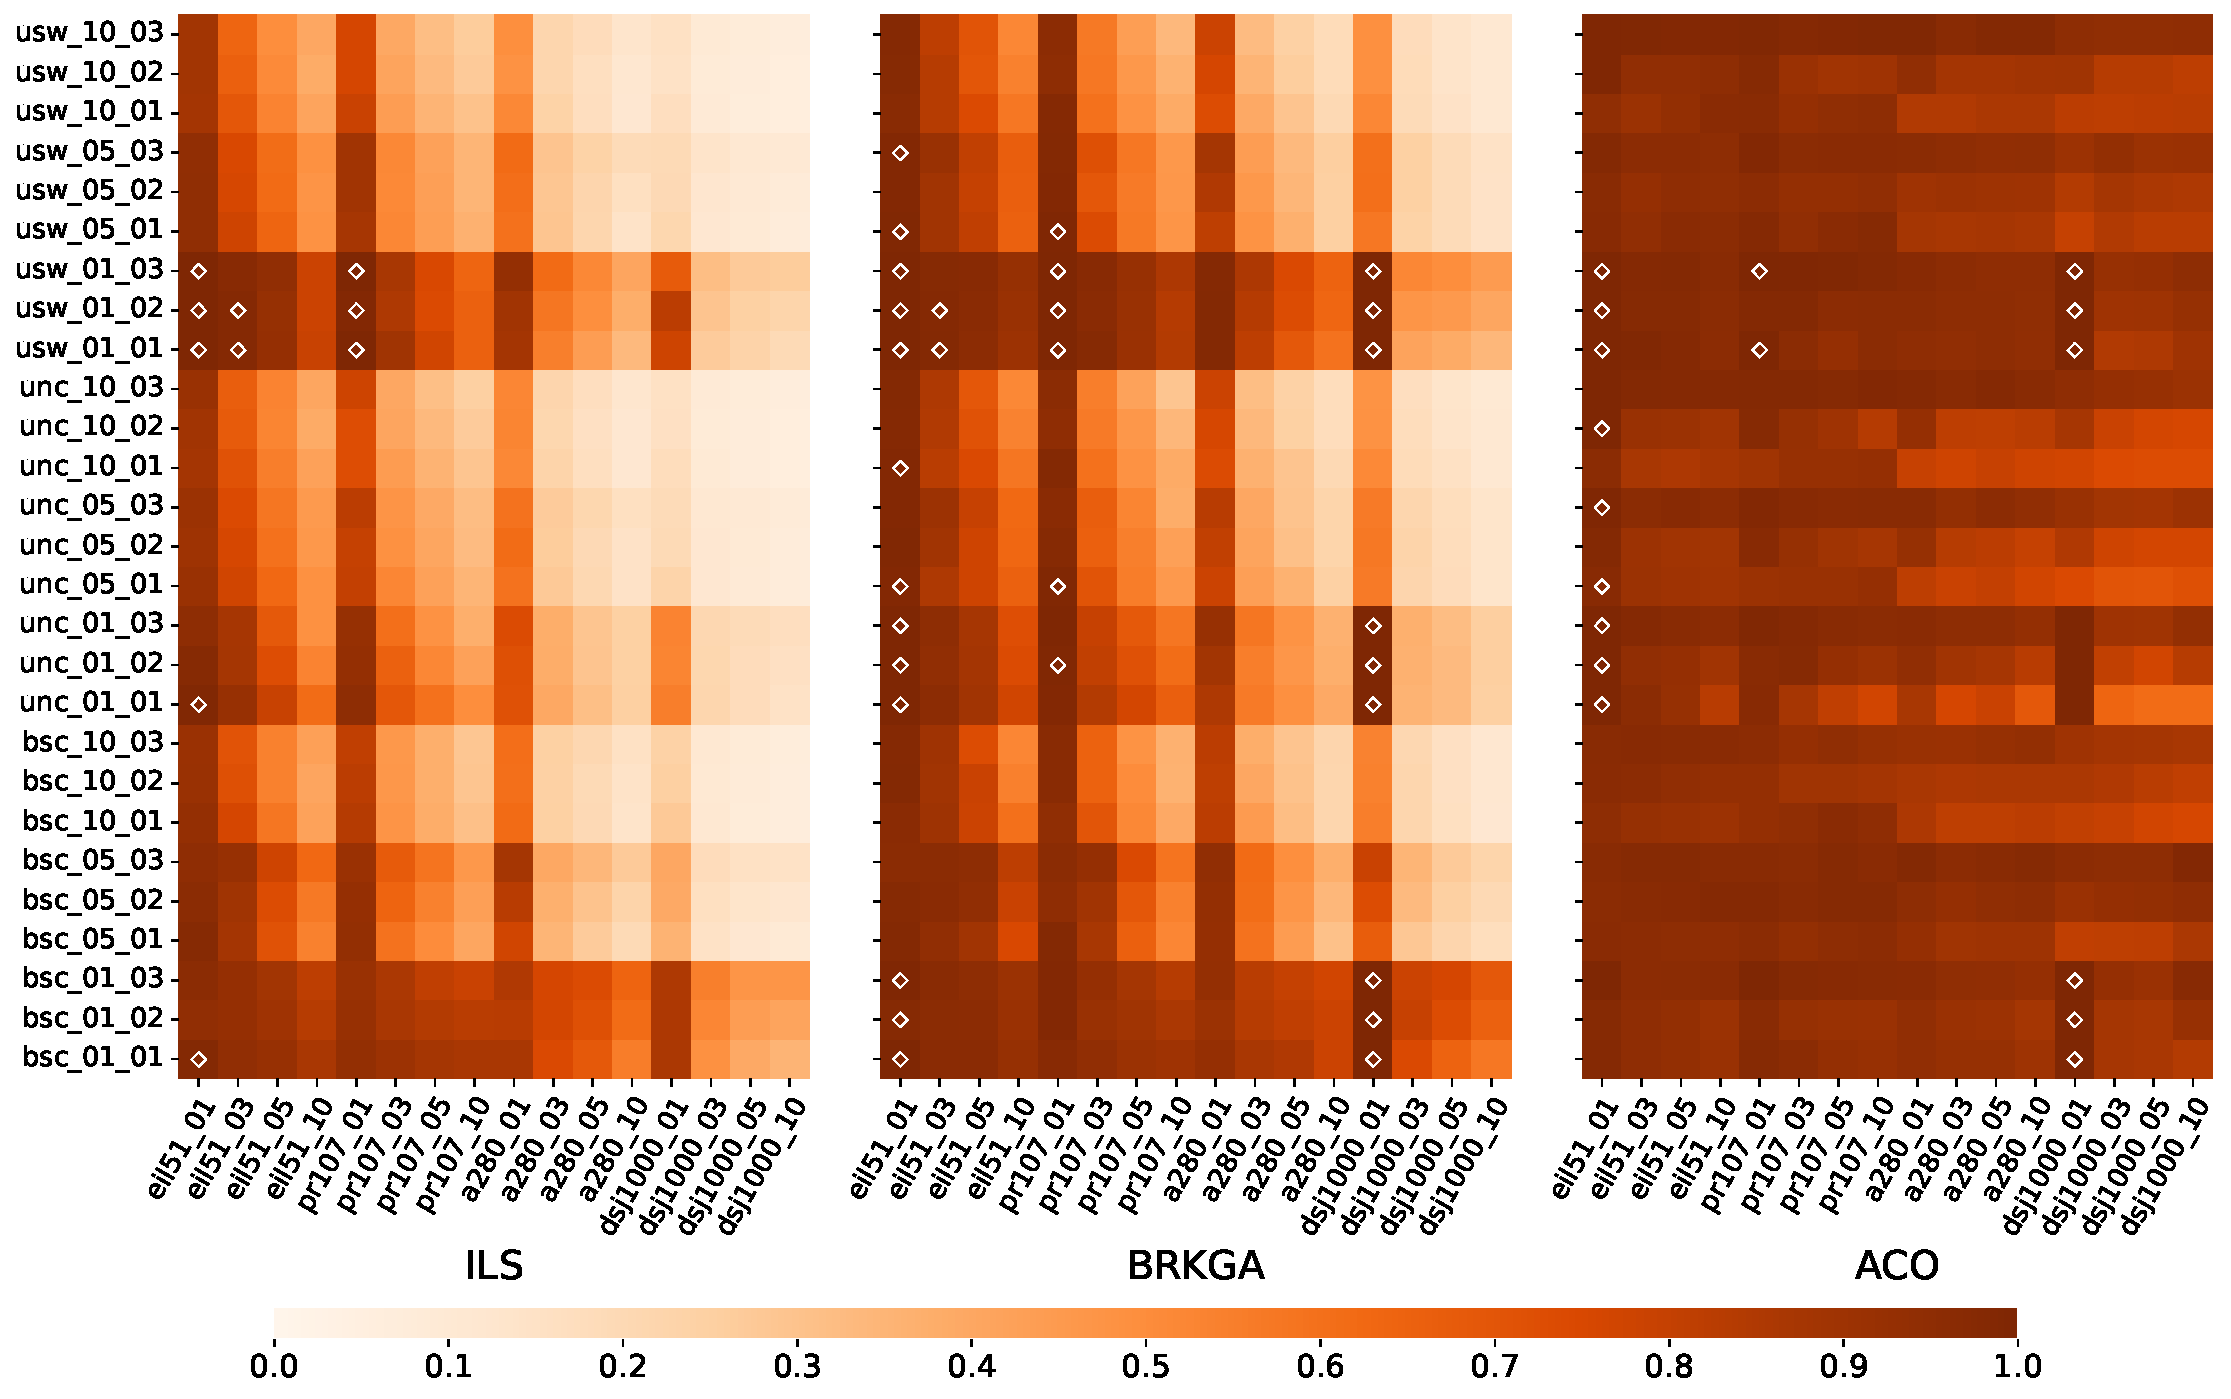
\includegraphics[width=0.95\linewidth]{img/profit_ratio_horizontal_1.pdf}
    \end{column}
\end{columns}
    % \centering
    % 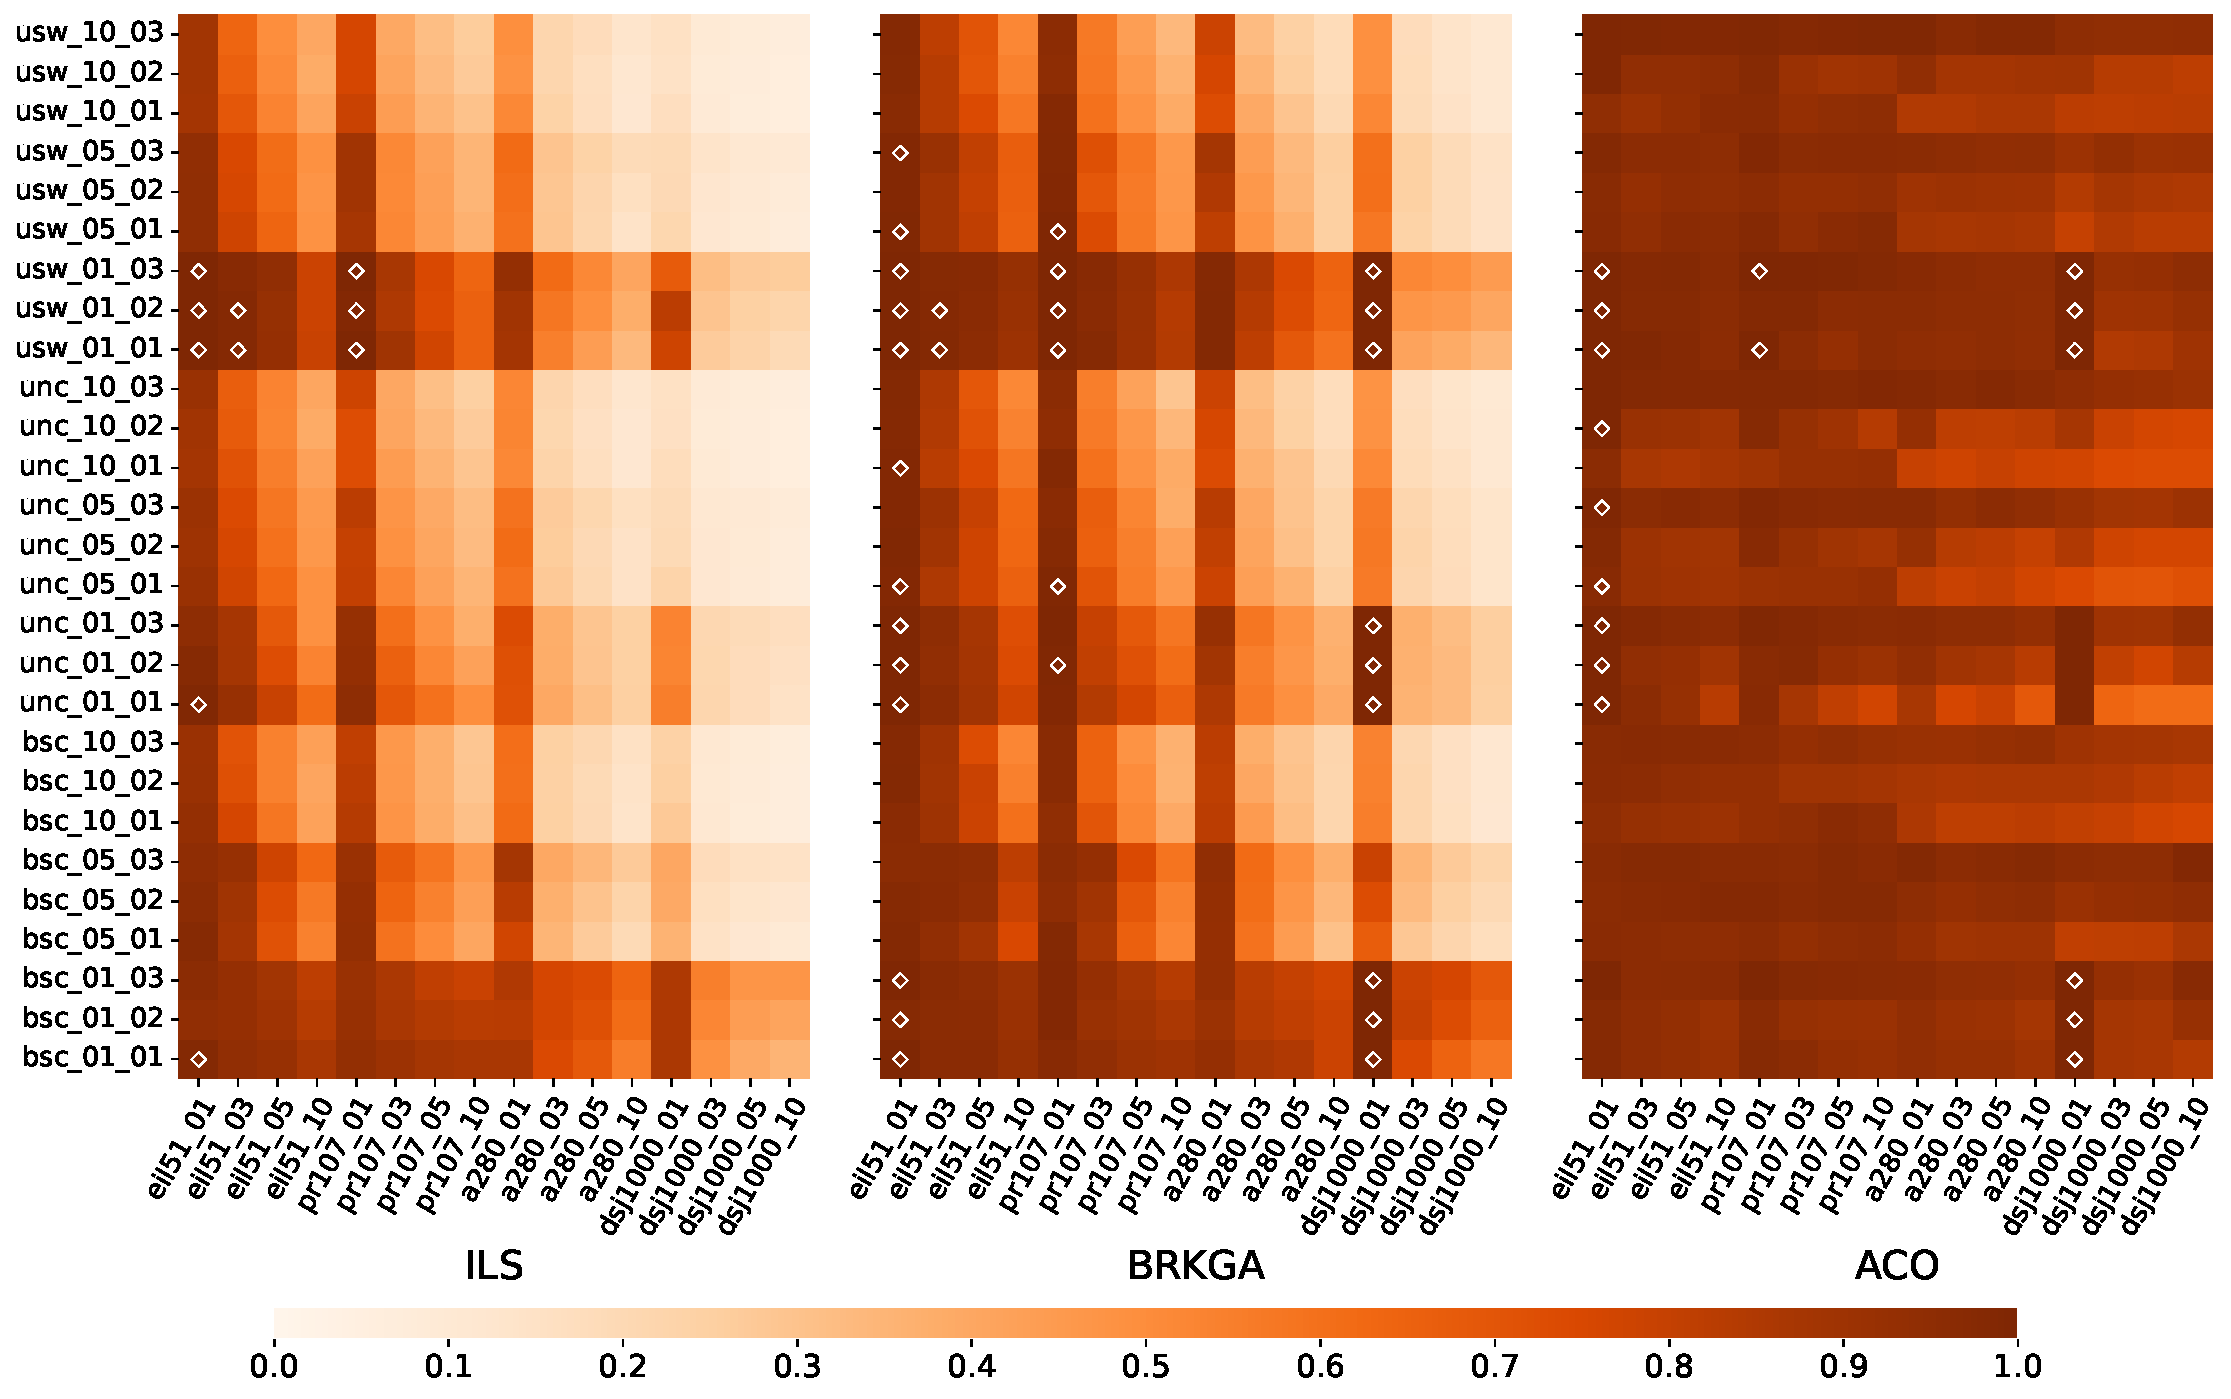
\includegraphics[width=0.7\linewidth]{img/profit_ratio_horizontal_1.pdf}
\end{frame}
\begin{frame}{Tỷ lệ xấp xỉ so với lời giải tốt nhất}
\begin{columns}
    \begin{column}{0.3\textwidth}
        \centering
        \begin{block}{\footnotesize Chú thích}
            \footnotesize 
            \begin{itemize}
                % \justifying
                \vspace{0.1cm}
                \item Mỗi ô là một trường hợp bài toán.
                \vspace{0.1cm}
                \item Hình thoi thể hiện tìm được lời giải tốt nhất trong thực nghiệm.
                \vspace{0.1cm}
                \item Càng nhiều hình thoi, thuật toán càng tốt.
                \vspace{0.1cm}
            \end{itemize}
        \end{block}
    \end{column}
    \begin{column}{0.6\textwidth}
        \centering
        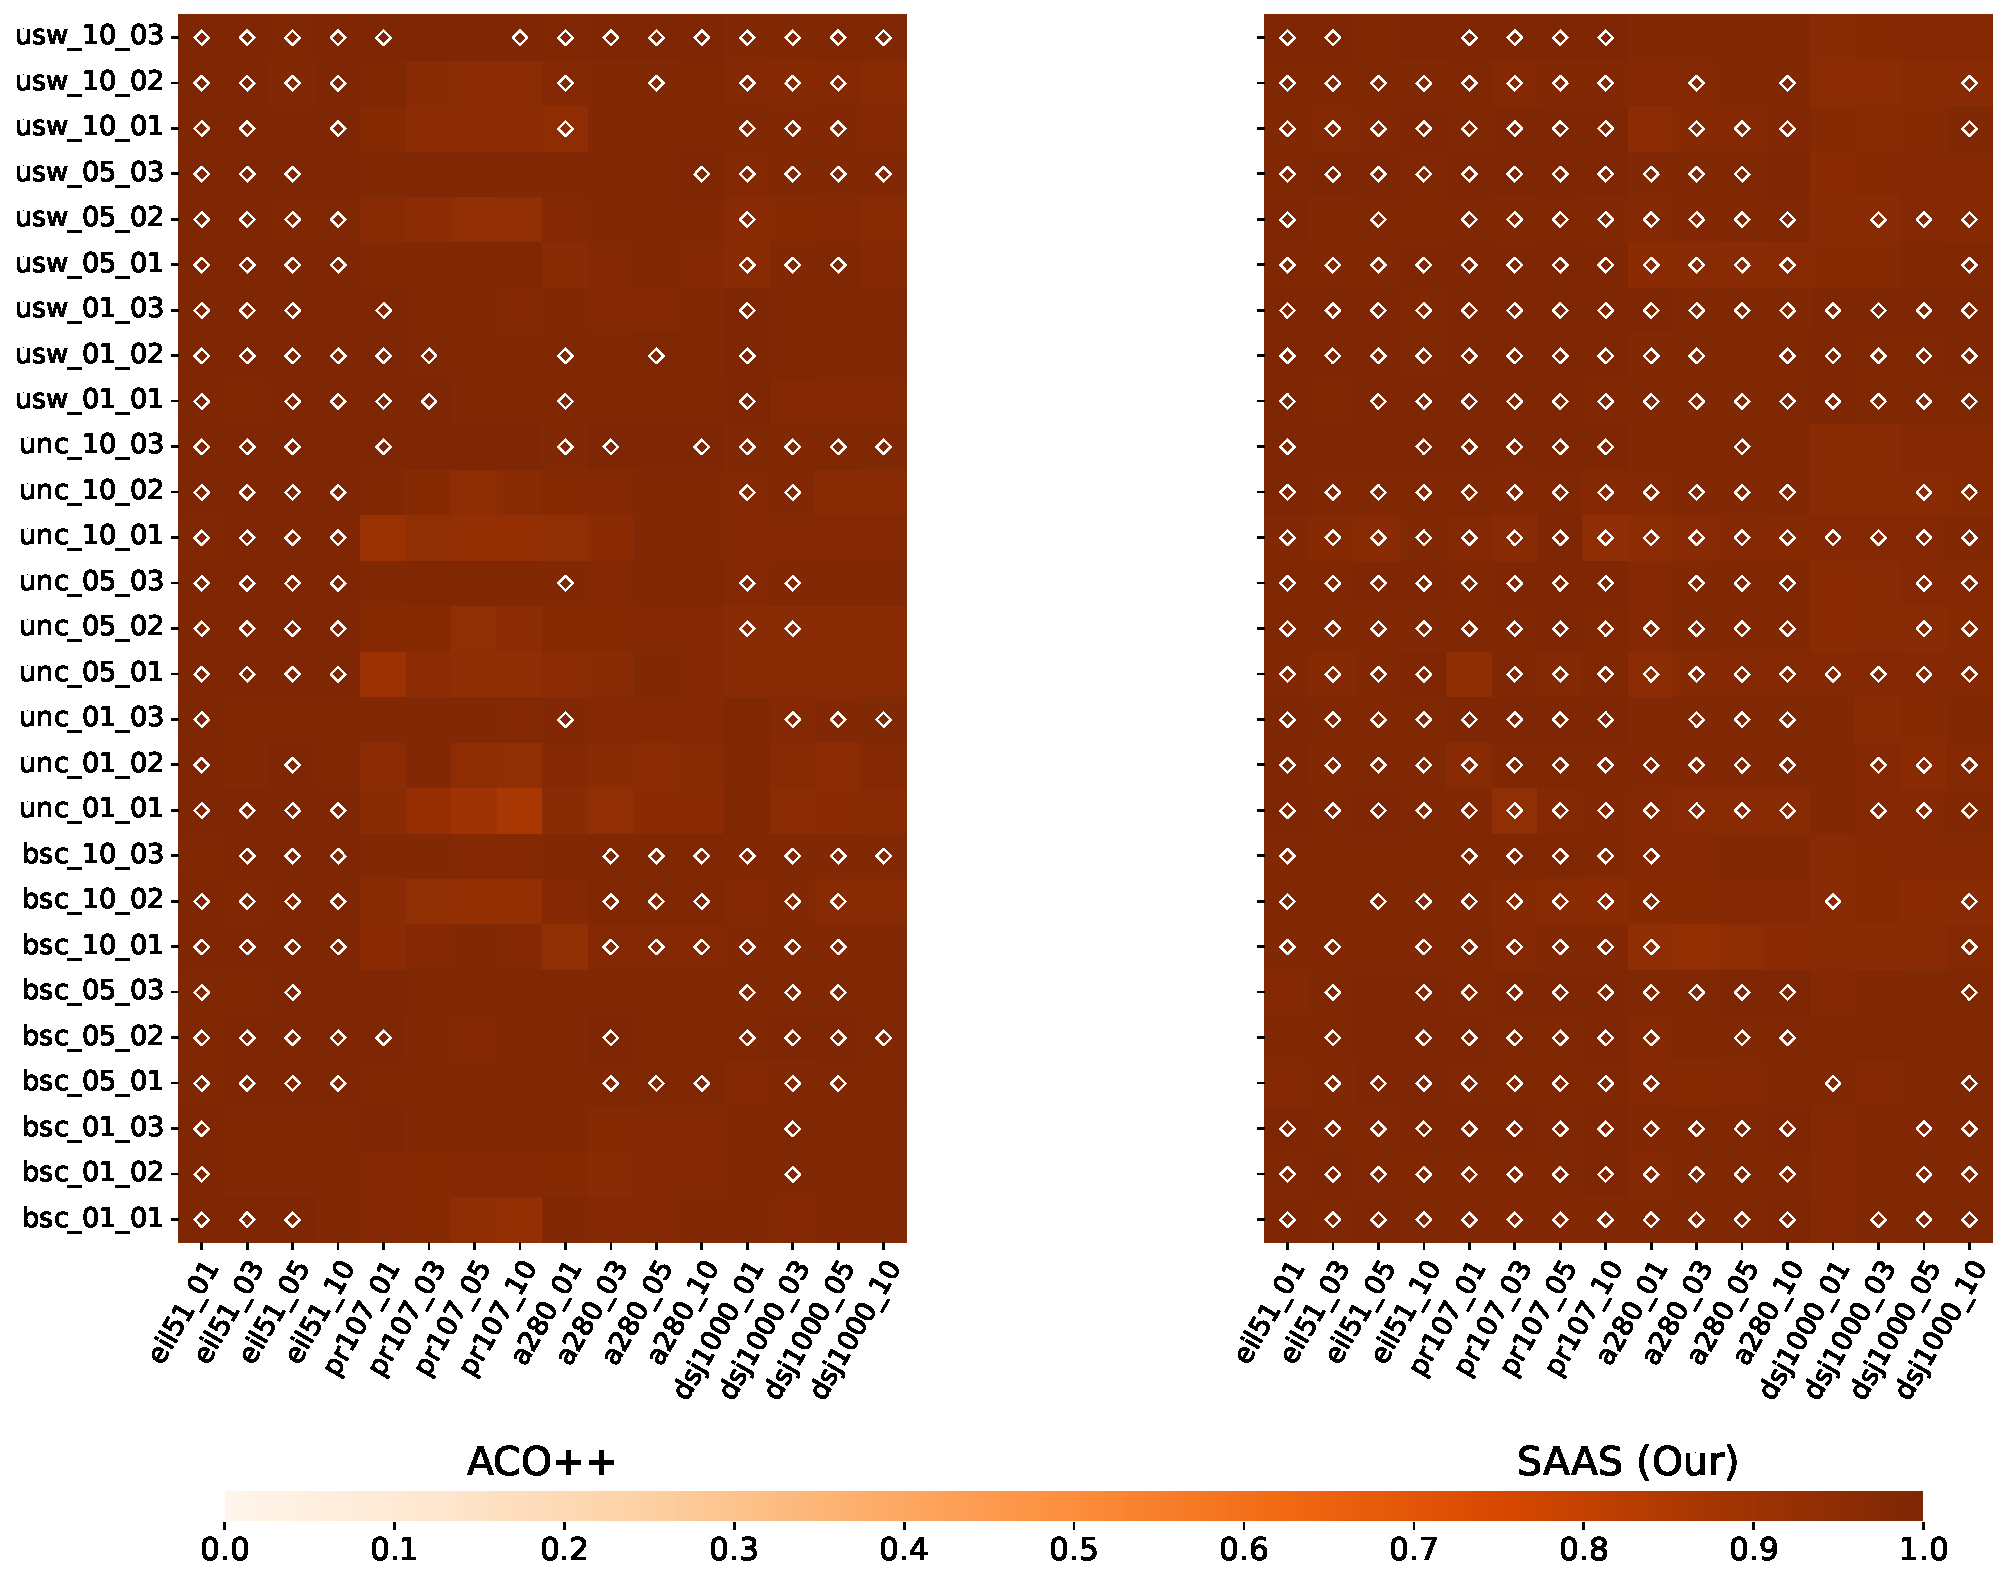
\includegraphics[width=\linewidth]{img/profit_ratio_horizontal_2.pdf}
    \end{column}
\end{columns}
    % \centering
    % 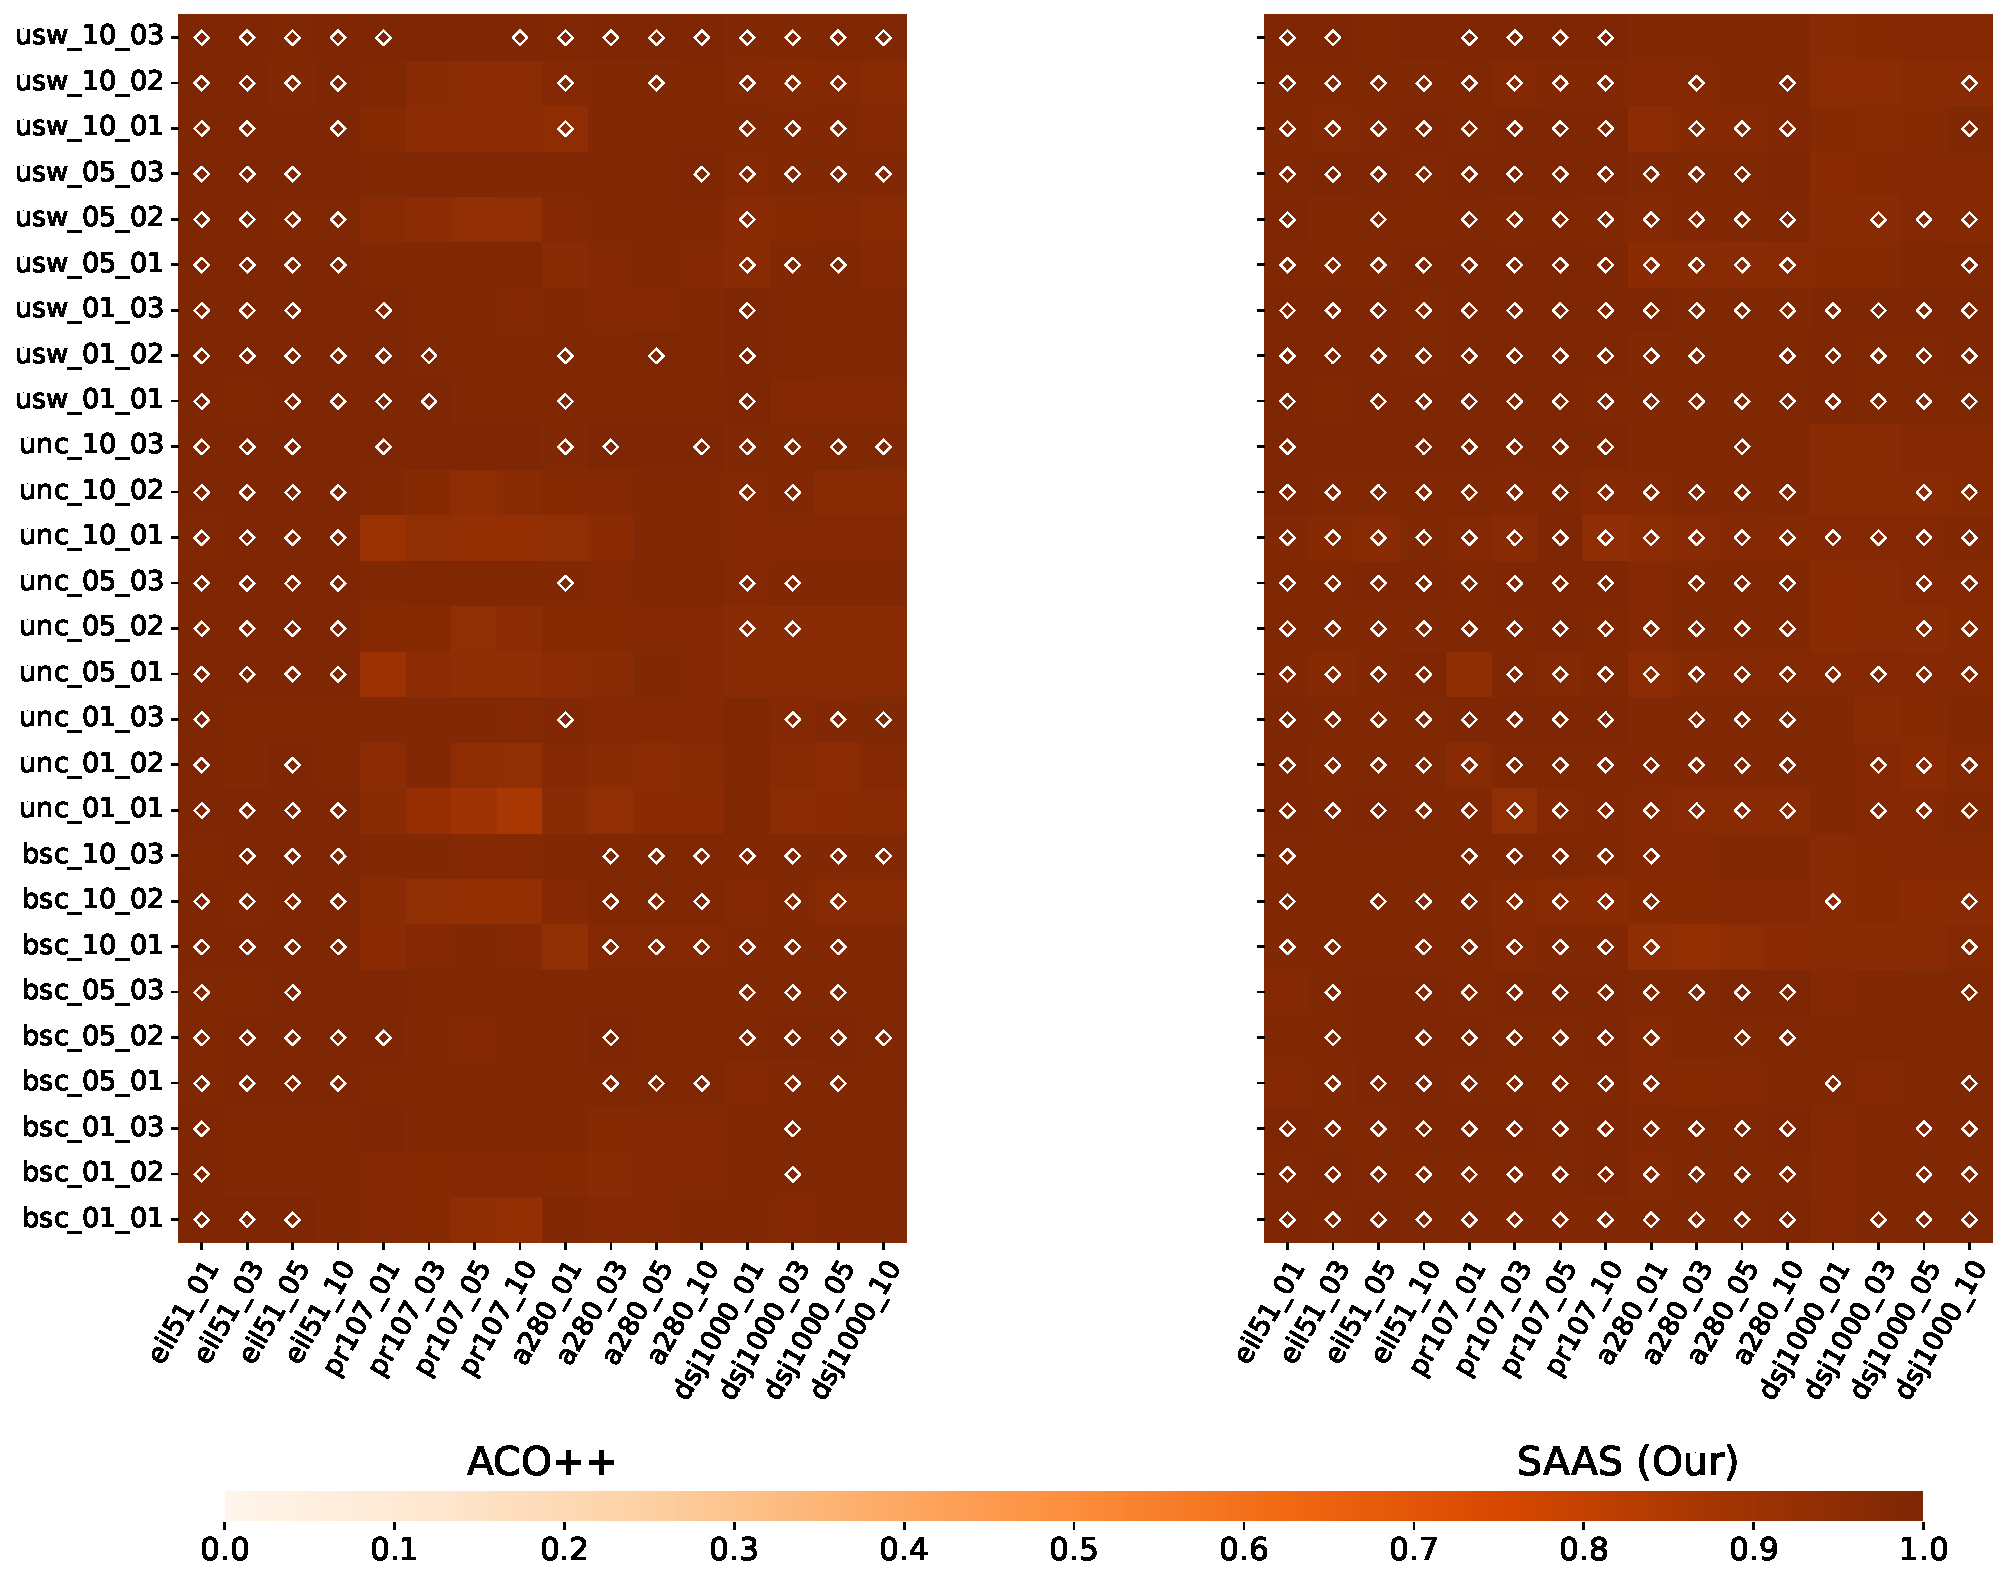
\includegraphics[width=0.6\linewidth]{img/profit_ratio_horizontal_2.pdf}
\end{frame}
\begin{frame}{So sánh hiệu suất thuật toán}
    \centering
    \begin{table}
        \small
        \caption{Tỷ lệ các trường hợp mà thuật toán i tìm ra giải pháp có chất lượng tốt hơn hoặc bằng thuật toán j}
        \label{tab:winpercent}
        \begin{tabular}{l|rrrrr}
            \hline
            i $\downarrow$ \ \ \ \ j $\rightarrow$ & ILS      & BRKGA   & ACO     & ACO++   & SAAS    \\
            \hline
            ILS                                    & -        & 2.55\%  & 4.40\%  & 2.55\%  & 2.31\%  \\
            BRKGA                                  & 100.00\% & -       & 16.20\% & 8.80\%  & 7.18\%  \\
            ACO                                    & 97.22\%  & 87.27\% & -       & 5.79\%  & 4.86\%  \\
            ACO++                                  & 99.54\%  & 95.83\% & 97.69\% & -       & 41.90\% \\
            SAAS (Ours)                            & 99.77\%  & 97.92\% & 98.61\% & 78.24\% & -       \\
            \hline
        \end{tabular}
    \end{table}
\end{frame}
\begin{frame}{So sánh chất lượng lời giải}
    \begin{figure}
        \centering
        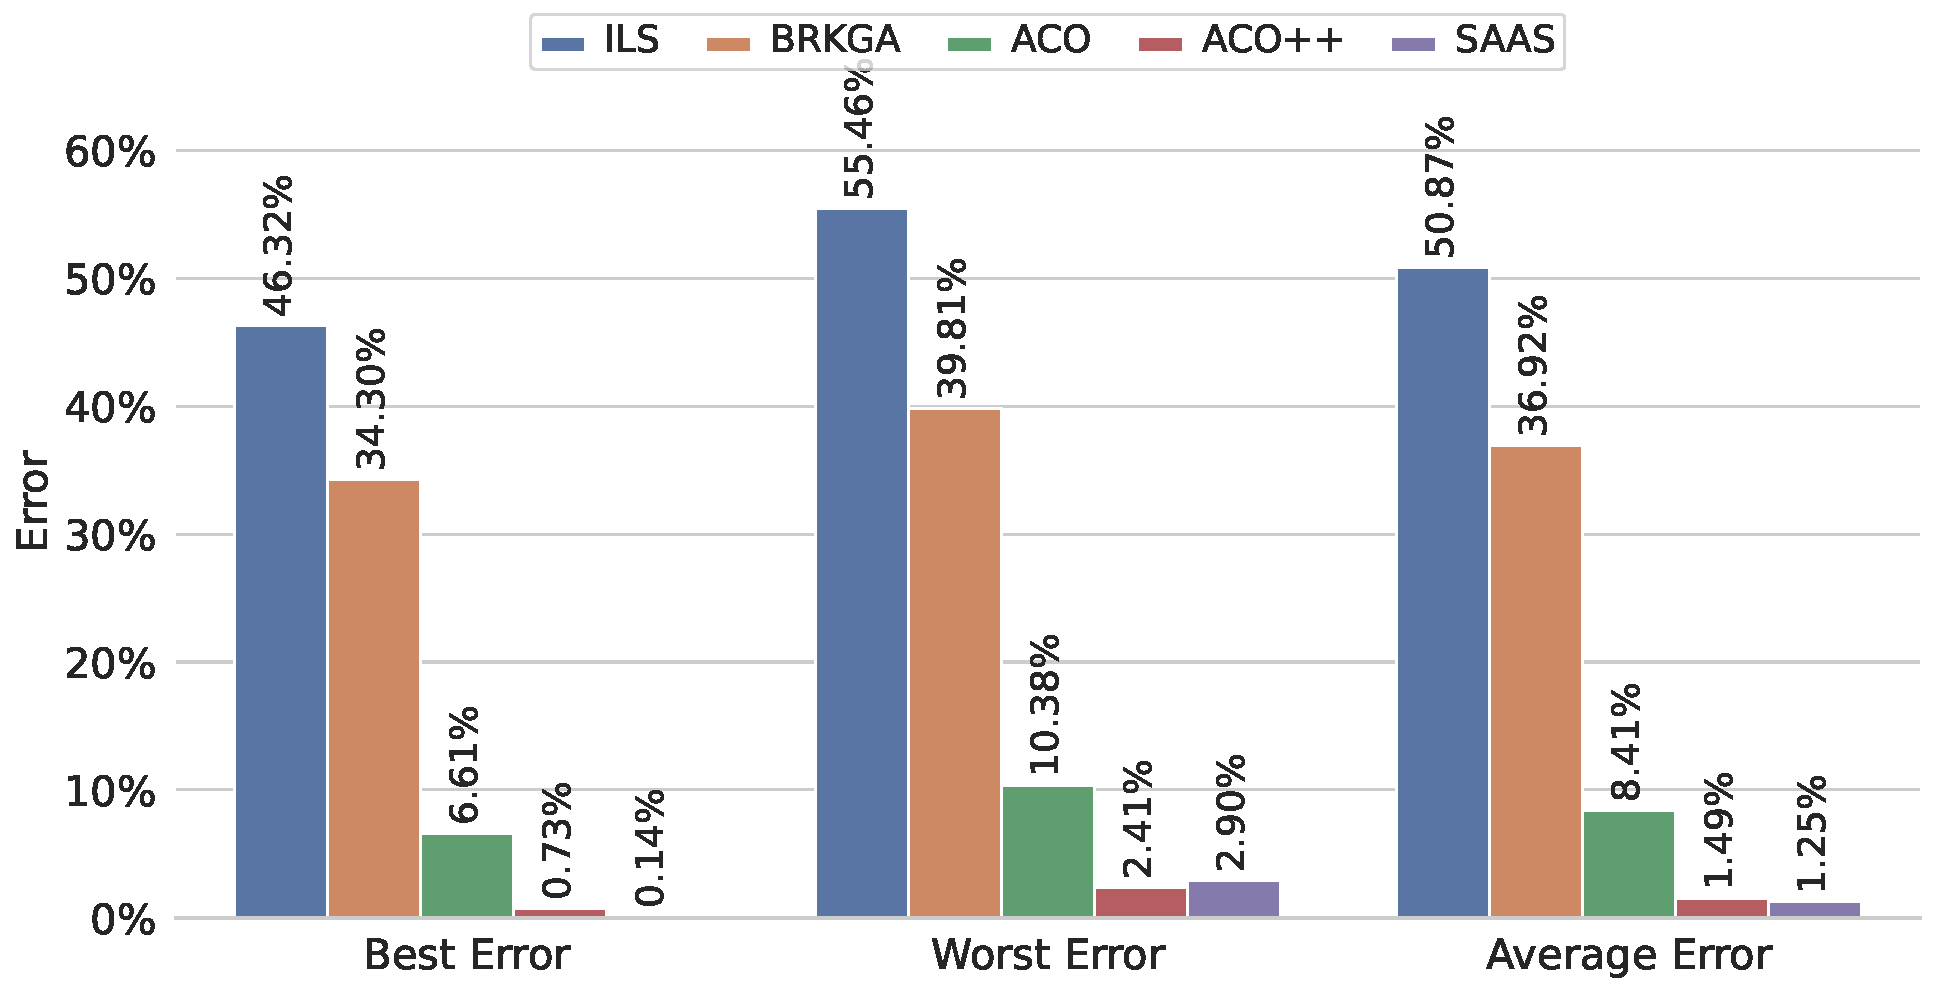
\includegraphics[width=0.75\linewidth]{img/error_rate.pdf}
        \caption{Độ lỗi trung bình qua toàn bộ benchmark. Thấp hơn là tốt hơn.}
        \label{fig:error_rate}
    \end{figure}
\end{frame}
\section{Kết luận}
\begin{frame}{Kết luận}
    \begin{block}{Kết luận}
        \begin{itemize}
            \vspace{0.1cm}
            \item Hai kỹ thuật kiểm soát tham số được tích hợp để cải thiện khả năng thích nghi và tính linh hoạt.
            \vspace{0.1cm}
            \item Kỹ thuật Bay hơi lười biếng giúp làm giảm độ phức tạp thời gian của giai đoạn bay hơi pheromone.
            \vspace{0.1cm}
            \item Phân cụm thứ bậc (hierarchical clustering) được tận dụng giúp làm giảm chi phí kiến chọn thành phố tiếp theo.
            \pause
            \vspace{0.1cm}
            \item Giải Thuật Đàn Kiến Tự Thích Ứng (SAAS) hiệu quả hơn ACO++ khi chỉ cần đúng một bộ siêu tham số để chạy toàn bộ benchmark.
            \vspace{0.1cm}
            \item SAAS cho thấy hiệu suất đáng chú ý khi vượt qua tất cả các thuật toán trước đây cho bài toán Điều Hướng Thu Thập (ThOP).
            \vspace{0.1cm}
        \end{itemize}
        \vspace{0.1cm}
    \end{block}
\end{frame}
\begin{frame}{Tài liệu tham khảo}
    \printbibliography
\end{frame}
\end{document}
